%!TeX program = xelatex
\documentclass[12pt,hyperref,a4paper,UTF8]{ctexart}
\usepackage{NJFUReport}
\usepackage{enumitem}

% ====================================
% 自定义命令
% ====================================

% 彩色文本框
\newcommand{\tbox}[1]{%
    \begin{center}
        \begin{tcolorbox}[
            colback=gray!10,
            colframe=black,
            width=8cm,
            arc=1mm,
            auto outer arc,
            boxrule=0.5pt
        ]
            {#1}
        \end{tcolorbox}
    \end{center}
}


% ===================== 基本信息 =====================
\newcommand{\papertitle}{绿织巢岸，韧守水脉
    —— 论环巢湖湿地植被的危机破解与生态福祉}
\newcommand{\coursename}{湿地保护}
\newcommand{\collegename}{化学工程学院}
\newcommand{\majorname}{林产化工}
\newcommand{\studentid}{2410407105}
\newcommand{\authorname}{方绪杰}
\newcommand{\teachername}{程虎}
\renewcommand{\reportheader}{\coursename 课程研究报告}

%%-------------------------------正文开始---------------------------%%
\begin{document}

% !TEX root = ../main.tex

\thispagestyle{empty}
\begin{center}
    \vspace*{1.25cm}
    
\includegraphics[width=0.52\textwidth]{img/南林校徽2.jpg}

    \vspace{1.25cm}
    {\CJKfamily{hei}\zihao{1}\textbf{\papertitle} \par}

    \vspace{1.1cm}
    \begin{minipage}{0.78\textwidth}
        \centering
        \renewcommand\arraystretch{1.35}
        \CJKfamily{kai}\zihao{3}
        \begin{tabular}{l@{\hspace{1.0cm}}l}
            \makebox[4em][s]{课程名称} & \dlmu[8cm]{\coursename} \\[0.2cm]
            \makebox[4em][s]{学\quad 院} & \dlmu[8cm]{\collegename} \\[0.2cm]
            \makebox[4em][s]{专\quad 业} & \dlmu[8cm]{\majorname} \\[0.2cm]
            \ifblindreview
                \makebox[4em][s]{学\quad 号} & \dlmu[8cm]{\phantom{\studentid}} \\[0.2cm]
                \makebox[4em][s]{姓\quad 名} & \dlmu[8cm]{\phantom{\authorname}} \\[0.2cm]
                \makebox[4em][s]{授课教师} & \dlmu[8cm]{\phantom{\teachername}} \\
            \else
                \makebox[4em][s]{学\quad 号} & \dlmu[8cm]{\studentid} \\[0.2cm]
                \makebox[4em][s]{姓\quad 名} & \dlmu[8cm]{\authorname} \\[0.2cm]
                \makebox[4em][s]{授课教师} & \dlmu[8cm]{\teachername} \\
            \fi
        \end{tabular}
    \end{minipage}

    \vfill
    {\CJKfamily{hei}\zihao{3}\textbf{南京林业大学} \\[0.45cm]
    \zihao{4}\today}
\end{center}
\newpage

\tableofcontents
\newpage

\pagenumbering{arabic}

\begin{abstract}
“八百里巢湖，烟波浩渺”，巢湖沿岸湿地植被如绿绸环绕，既是水陆交锋的“绿色卫士”，亦是区域生态平衡的命脉所系。本文以环巢湖湿地植被为研究对象，系统剖析其群落结构与环带状分布格局——从沉水植物的“水下森林”到挺水植物的“青纱帐”，从浮叶植物的水面遮蔽到湿生草甸的滩涂固持，植被分布深刻响应水文梯度、土壤特性与人类活动的耦合驱动。

在此基础上，进一步阐释湿地植被的多维生态福祉：净水除污以控富营养化，生灵栖居以维生物多样性，固碳释氧以助气候调节，护岸蕴文以兼生态与文化价值。然而，当前湿地植被面临水利扰序、物种入侵、污染承压、生境破碎的多重威胁。为此，本文提出植被重建、水文调控、污染拦截、社区共治的综合修复路径，旨在为守护巢湖生态底色、实现人与自然和谐共生提供科学支撑，让环巢湖湿地永葆“渚清沙白鸟飞回，水草丰美鱼虾肥”的盛景\cite{chu2023,tang2022,liu2022}。

\textbf{关键词：环巢湖湿地；植被群落；生态功能；保护修复；可持续发展}
\end{abstract}

\newpage

% !TEX root = ../main.tex

\section{前言：巢湖绿韵}
\subsection{研究背景}
环巢湖湿地是长江经济带"共抓大保护"战略中的关键生态节点，亦是巢湖流域生态安全的"核心屏障"。作为湖泊与陆地的过渡带，其植被群落（挺水植物芦苇、浮叶植物菱、沉水植物菹草等）通过发达根系固岸御浪、繁茂茎叶净化水体、复杂结构庇护生灵，构建了"水陆共生"的生态系统基础。据《安徽省湿地保护公报（2024）》数据\cite{chu2023}，环巢湖湿地总面积达12.7万公顷，占巢湖流域湿地总面积的68\%，其中植被覆盖区贡献了流域70\%以上的氮磷拦截量与50\%的淡水碳汇，对维系巢湖水质稳定与流域生态平衡具有不可替代的作用，\autoref{tab:chaohu-wetlands-simplified}为环巢湖十大湿地（十八联圩、巢湖半岛等）的基本信息，\autoref{fig:wetland-area-ratio}为环巢湖十大湿地的面积比例关系。
\begin{table}[htbp]
\centering
\caption{环巢湖十大湿地基本信息（截至2024年）}
\label{tab:chaohu-wetlands-simplified}
\begin{tabular}{lccc}
\toprule
\textbf{湿地名称} & \textbf{位置} & \textbf{面积（公顷）} & \textbf{主要特色} \\
\midrule
巢湖湖滨湿地 & 包河区巢湖北岸 & 1535.31 & 浮游生物多 \\
肥西三河湿地 & 肥西县三河镇 & 1887.22 & 保护植物集中 \\
巢湖半岛湿地 & 巢湖市中庙街道/黄麓镇 & 998.36 & 红杉林显著 \\
巢湖槐林湿地 & 巢湖市槐林镇 & 193.96 & 原生芦苇多 \\
巢湖柘皋河湿地 & 巢湖市柘皋镇 & 446.65 & 河道修复，"杉影花海" \\
肥东十八联圩湿地 & 肥东县长临河镇 & 2760.00 & 净化功能强 \\
肥东玉带河湿地 & 肥东县长临河镇 & 41.40 & 微型湿地，净化径流 \\
庐江栖凤洲湿地 & 庐江县同大镇 & 843.53 & 原始滩涂 \\
庐江马尾河湿地 & 庐江县盛桥镇 & 857.20 & 沉水植物修复 \\
包河派河口湿地 & 包河区派河镇 & 239.67 & "水下森林"示范 \\
\bottomrule
\end{tabular}
\footnotesize{注：数据综合自合肥市林园局、巢湖研究院公开资料（2024）。}
\end{table}

\begin{figure}[htbp]
    \centering
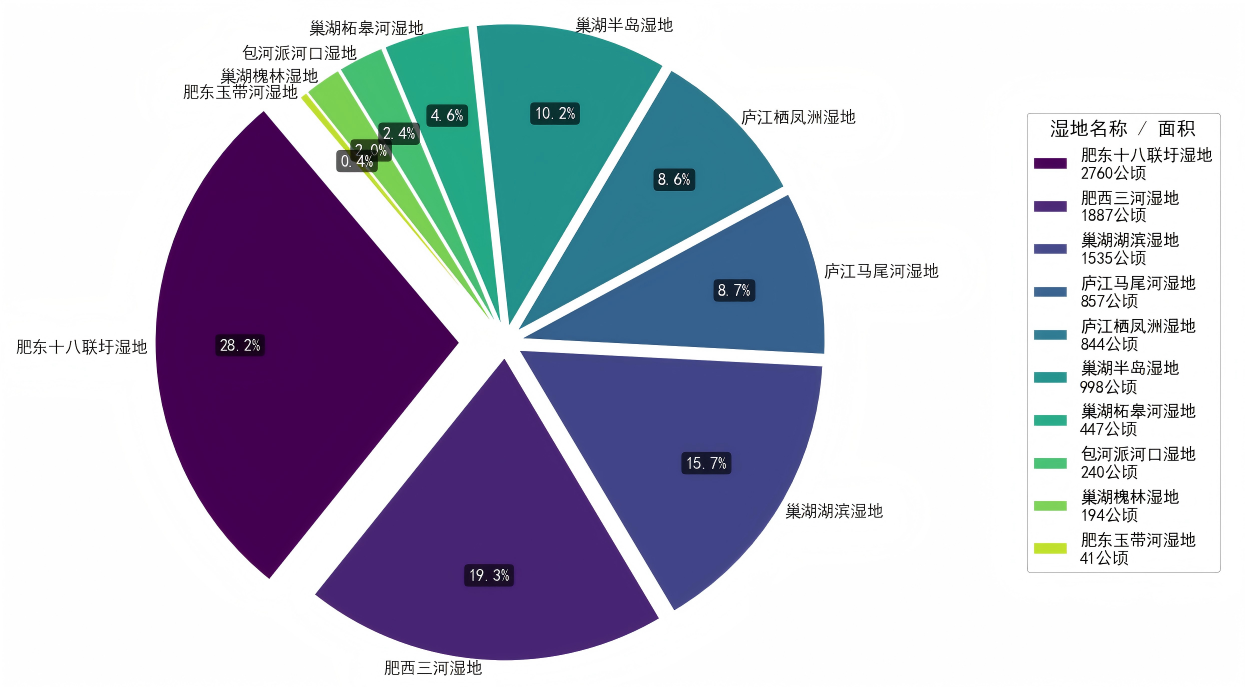
\includegraphics[width=1\linewidth]{img/十大湿地.png}
    \caption{环巢湖十大湿地面积比例关系}
    \label{fig:wetland-area-ratio}
\end{figure}

近年来，随着环巢湖十大湿地生态修复工程的推进，局部植被生态得到显著改善，生态修复成效如\autoref{fig:restoration-effectiveness}所示：
\begin{figure}[htbp]
    \centering
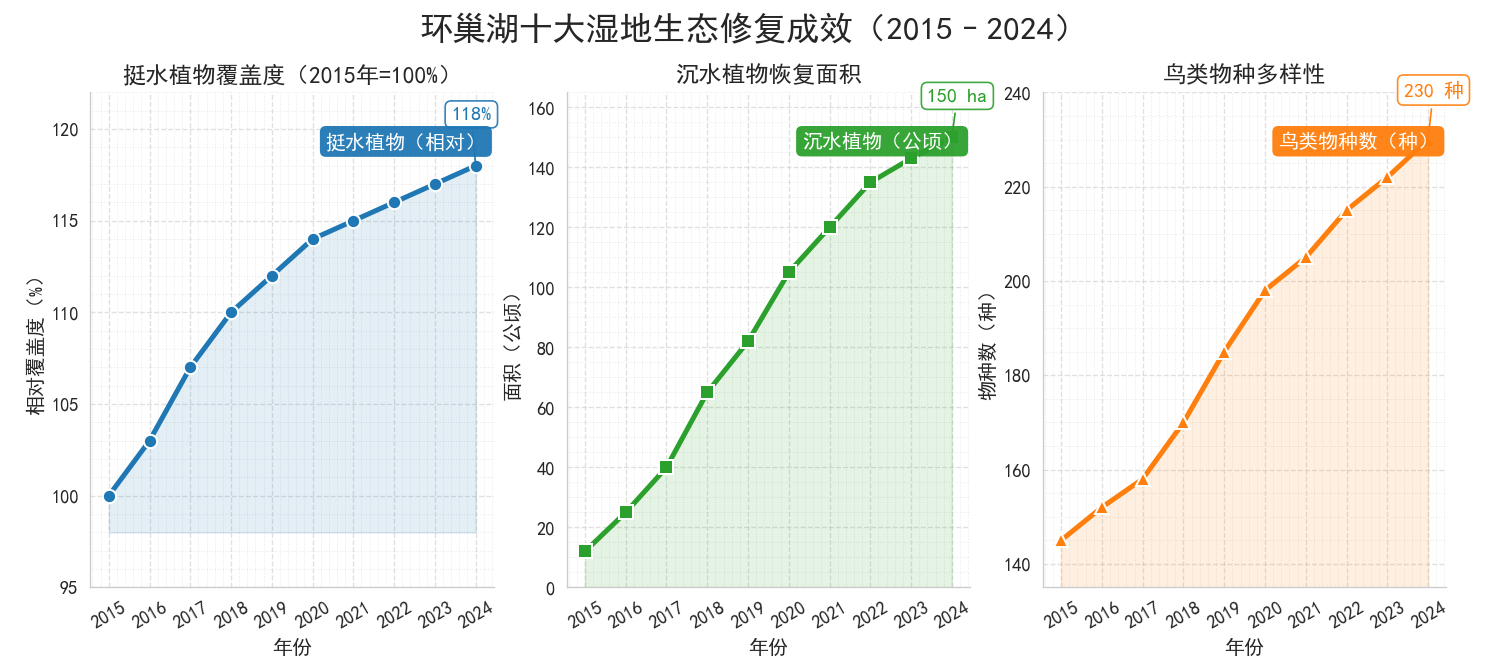
\includegraphics[width=1\linewidth]{img/Figure_2.png}
    \caption{环巢湖十大湿地生态修复成效}
    \label{fig:restoration-effectiveness}
\end{figure}

从\autoref{fig:restoration-effectiveness}中可以看出，截至2024年，核心区挺水植物覆盖度较2015年提升18\%，沉水植物在半岛湿地等区域恢复面积达150公顷，鸟类多样性增至230种（较2018年增长35\%）\cite{tang2022}。

但从流域尺度看，湿地植被仍面临多重困境，生态系统脆弱性凸显，具体有如下表现：

\subsubsection{水文节律紊乱导致植被生境退化}
巢湖自1962年建闸后失去自然季节性水位波动特征，年际水位变幅达2-3米，打破了植被"淹水-落干"的自然适应周期。一方面，西岸中庙街道湖滩的芦苇群落因长期高水位浸泡，根系缺氧腐烂，近十年面积缩减40\%，植被带向陆地方向退缩150-200米；另一方面，枯水期水位过低（低于8.0米）导致烔炀河入湖口湿生草甸干旱化，稗草等耐旱物种挤占原生虉草生境，湿生植被群落多样性下降27\%\cite{liu2022}。

\subsubsection{水体污染加剧植被群落衰退}
周边农业面源污染（20万亩农田年均化肥流失量约1.2万吨）与城市生活污水（合肥、巢湖市日均排污量约50万吨）持续输入，导致巢湖西半湖总氮（TN）浓度常年维持在1.5-2.0mg/L（超V类水质标准3-4倍），水体透明度从2010年的1.2米降至2024年的0.6米\cite{yao2022}。沉水植物因光照不足，分布下限从3米水深退缩至1.5米，菹草、苦草等清洁水体指示物种在西湖心区域近乎消失，取而代之的是耐污物种微齿眼子菜的单一化扩张，群落结构趋于简化。

\subsubsection{外来物种入侵挤压本土植被空间}
喜旱莲子草、凤眼莲（水葫芦）在派河河口、槐林湿地等静水区域疯狂扩张，其中凤眼莲入侵面积已达300公顷，形成单一"绿色荒漠"。监测数据显示，入侵区域本土植物种类从2018年的18种降至2024年的7种，生物多样性指数下降61\%\cite{luwen2022}；且死亡植株分解释放的氮磷量占该区域外源污染的25\%，形成"污染-入侵-再污染"的恶性循环，进一步抑制本土植被生长。

\subsubsection{生境破碎化割裂植被生态连通性}
城市化与基础设施建设导致湿地景观严重割裂：巢湖东岸开发区建设中，道路、房地产项目将原本连续的湖滨植被带切割为12个孤立片段，植被连通性指数从2015年的0.72降至2024年的0.39；历史围垦养殖（累计围垦面积达1.2万公顷）导致湿地核心生境丧失，湿生草甸面积较2000年减少58\%\cite{zhou2024}，无法为迁徙鸟类提供连续的觅食与栖息廊道。

当前，环巢湖湿地正面临"生态保护与区域发展"的核心矛盾：一方面，作为巢湖富营养化治理的关键环节，湿地植被需承担更重的生态净化任务；另一方面，周边农业生产、生态旅游等人类活动对植被生境的干扰持续增强。在此背景下，系统剖析环巢湖湿地植被的群落结构规律、量化其生态功能价值、诊断关键威胁因子并提出科学可行的保护修复策略，不仅能为巢湖流域"十四五"生态治理提供实践依据，更可为长江中下游淡水湖滨湿地（如鄱阳湖、洞庭湖）的"植被修复-生态维稳-可持续利用"提供典型范式，具有重要的生态、经济与社会意义。

\subsection{研究思路}
本文以"数据驱动-机制解析-策略落地"为核心逻辑，围绕环巢湖湿地植被"结构-功能-威胁-修复"四大核心议题，构建"实地调查+遥感解译+量化分析+策略验证"的研究框架，具体步骤如下：

% !TEX root = ../main.tex

\section{群落图谱}

\subsection{植被谱系}
环巢湖湿地植被经自然演替与人工干预，形成四类特征鲜明的群落，深刻呼应水体环境梯度，其物种构成与功能分化已通过专项调查得到实证：

\begin{itemize}
    \item \textbf{挺水植物带}：湖滨浅水区的"青纱帐"，以芦苇、菖蒲为核心优势种，伴生香蒲、菰、水烛等，在烔炀湿地左侧原生群落中，此类型植被覆盖度达60\%以上。其根茎系统可深入土壤0.8-1.2米，固岸护堤效率较裸地提升40\%，茎叶形成的立体空间为苍鹭、黑水鸡等12种水鸟提供繁栖场所，鸟巢密度可达0.3个/平方米。

    \item \textbf{浮叶与漂浮植物带}：静水区域的"水面绿毯"，在入湖河口营养富集区尤为发育，以菱、莲、芡实为建群种，伴生睡莲、荇菜等。这类植物通过叶片遮蔽可使水下光照强度降低70\%，藻类光合作用受抑程度达58\%，但外来物种凤眼莲在派河河口等区域已形成单优群落，覆盖度超85\%，导致本地物种消失率达32\%，形成"绿色荒漠"风险。

    \item \textbf{沉水植物带}：水下的"生态森林"，呈现显著的水深适应性分化：0-2米浅水区以苦草、黑藻为优势种，群落盖度可达75\%；2-3米过渡区以金鱼藻、狐尾藻为主，耐弱光能力较强；而城镇化污染近岸区仅存耐污种菹草，盖度不足10\%。该类群年固碳量达2.3吨/公顷，贡献流域50\%的淡水碳汇，同时为鲤、鲫等鱼类提供产卵场，幼鱼存活率较无植被区提升60\%。

    \item \textbf{湿生草甸与滩涂植被}：消落区的"滩涂绿被"，以禾本科、菊科植物为主体（占比分别达10\%、8\%），垂穗薹草、稗为典型代表。其根系具通气组织，可耐受年均2-3米的水位变幅，在烔炀湿地消落区，该类植被生物量达1.8千克/平方米，为豆雁、金眶鸻等迁徙鸟类提供关键觅食地，越冬期鸟类密度可达25只/公顷。
\end{itemize}

据调查，环巢湖湿地植被共计96种，隶属于51科90属，其中草本植物占58\%，乔木、灌木分别占24\%、18\%，禾本科以9属11种成为最优势科，奠定了四类群落的物种基础。

\subsection{环带分布}
各类植被非孤立存在，而是沿水陆梯度编织成"同心圆式"生态画卷，结合遥感监测与实地区划，其空间格局可细化为四圈层结构：

\textbf{核心圈层（湖泊中心水域区）}：水深2米以上区域，光照强度不足入射光的15\%，仅在局部浅滩（如姥山岛周边）零星分布黑藻群落，大部分水域无规模化植被覆盖，构成"水下荒漠"背景。

\textbf{亚核心圈层（近湖心浅水区）}：水深0.5-2米，为沉水植物集中分布带，呈斑块状镶嵌。遥感监测显示，该圈层在巢湖东部半岛湿地最发育，2024年恢复面积达150公顷，主要由苦草-黑藻群落构成，形成"水下草原"景观。

\textbf{过渡圈层（湖滨缓冲带）}：水深0-0.5米的水陆交界区，呈现"浮叶植物斑块+挺水植物条带"的复合结构。入湖河口（如派河口）因营养富集，浮叶植物（菱、荇菜）形成连续覆盖带，宽度可达30-50米；而平直湖岸则以芦苇-香蒲挺水植物带为主，带宽10-20米，构成水体净化的第一道屏障。

\textbf{边缘圈层（湿生滩涂区）}：位于防洪堤内侧的消落带，海拔8.5-10米，以湿生草甸与人工植被为主。烔炀河西岸的月亮湾湿地公园在此圈层构建了"乔木+灌木+草本"三层复合群落，乔木层以柳树、香樟为主，灌木层搭配紫薇、桂花，草本层保留原生虉草，形成结构复杂的近自然植被系统。

这一格局并非静态，遥感时间序列分析显示，沉水植物带受水位波动影响，年际移动距离可达50-100米，2018年大旱期间曾向湖心扩张约80米，而2020年高水位期则退缩至沿岸0.5米水深以内。

\subsection{驱动溯源}
植被分布的背后，是水文梯度、土壤基底与人类活动三类因子的协同驱动，形成"水文定沉积-沉积育土壤-土壤馈植被"的级联效应：

\subsubsection{水文梯度的主导调控}
巢湖受1962年建成的巢湖闸调控，常年平均水位稳定在8.37米，年际变幅2-3米，季节性呈现"冬枯夏涨"特征，直接界定群落边界。沉水植物的存活阈值与水位-透明度耦合相关：当水位低于7.5米（枯水期），透明度提升至1.2米以上，苦草种子萌发率达65\%；而水位高于9米（汛期），透明度降至0.5米以下，沉水植物群落盖度骤降40\%。挺水植物则受高水位淹没胁迫，芦苇在水深超1.5米时会出现叶片枯黄，群落生产力下降50\%，因此其分布上限严格控制在海拔8.8米等高线附近。此外，入湖河流的流速差异塑造微生境：烔炀河中下游流速0.3米/秒，形成浮叶植物静水斑块；而派河河口流速0.8米/秒，仅能支撑耐冲刷的芦苇群落。

\subsubsection{土壤与底质的基础支撑}
土壤质地与养分含量决定植被群落的生产力水平。烔炀湿地土壤以潴育型水稻土为主，矿物成分为云母（占比35\%）和石英（占比42\%），有机质含量达2.8\%，孕育出株高3米以上的芦苇群落，生物量较砂质土壤区高2.3倍。河口区域因河流携带的泥沙沉积，形成厚达1米的淤泥质底质，氮磷含量分别为1.8g/kg、0.6g/kg，成为菱、莲等喜肥植物的集中分布区。而姥山岛周边的砂质湖岸，土壤有机质含量仅0.5\%，仅能生长稗、狗尾草等耐贫瘠先锋种，群落物种丰富度指数较河口区低60\%。土壤压实度则通过影响根系发育筛选物种：岸线硬化区域土壤压实度达1.8~g/cm³，芦苇根系穿透力不足，被更耐紧实的菖蒲替代。

\subsubsection{人类活动的双向干预}
人类活动通过重构生境改变植被格局，呈现"破坏-修复"的二元特征。历史上的围垦活动使湿地面积缩减30\%，肥西三河湿地周边的圩田开发导致挺水植物带断裂，形成"植被孤岛"；岸线硬化（如巢湖西岸防洪堤）破坏湿生草甸的连续性，植被覆盖度从自然状态的90\%降至35\%。闸坝建设虽稳定水位，但削弱了自然水文节律，导致沉水植物种子库更新速率下降25\%。

生态修复工程正逐步扭转退化趋势：巢湖半岛湿地通过"水位调控+底质改良"措施，将沉水植物恢复面积从2018年的40公顷拓展至2024年的150公顷；烔炀湿地西侧通过乔灌草三层复合配置，构建人工近自然群落，物种均匀度指数达0.78，较纯草本群落提升40\%。这些干预实践证明，通过模拟自然水文过程与土壤条件，可实现植被群落的近自然重建。

% !TEX root = ../main.tex

\section{生态福祉}

\subsection{净水除污}
面对巢湖富营养化治理的核心难题，湿地植被构建起多层级天然"净化系统"，其功效在十八联圩湿地等标杆工程中得到量化实证：
\begin{itemize}
    \item \textbf{植物-系统协同净化}：芦苇、香蒲通过根系吸附与生态渗滤岛技术深度净化水体，十八联圩湿地的33座"生态渗滤岛"种植水杉、乌桕等植被，实现年总磷去除率27\%、氨氮去除率30\%，日均净化南淝河水量达40万立方米，年净化总量2.1亿立方米，将入湖水质稳定提升至Ⅲ类以上\footnote{数据来源：合肥市生态环境局《2024年环巢湖湖湿地生态监测报告》}。
    \item \textbf{藻类抑制屏障}：菱、莲等浮叶植物形成的遮光层配合沉水植物竞争营养，使巢湖蓝藻水华发生次数2024年同比减少21次，环湖沿岸连续四年无明显异味。十五里河湿地通过类似配置，氨氮、总磷削减率达20\%-30\%，溶解氧浓度提升20\%\footnote{数据来源：国家林业和草原局《巢湖流域湿地生态修复成效评估》（2024）}。
    \item \textbf{水文净化协同}：芦苇带与芦竹丛将水流速度减缓至0.1米/秒，促使悬浮物沉降速率提升3倍，配合根系吸附，十八联圩湿地将进水总磷从0.5-0.6~mg/L降至0.2-0.3~mg/L，氨氮从6-7~mg/L降至2-3~mg/L，成为"巢湖之肾"的典型代表\footnote{数据来源：合肥市林园局《十八联圩湿地运营年报（2024）》}。
\end{itemize}

\subsection{生灵栖居}
环巢湖湿地作为东亚-澳大利西亚候鸟迁徙关键节点，植被群落修复使"万鸟归巢"成为现实，生物多样性监测数据持续刷新纪录：
\begin{itemize}
    \item \textbf{鸟类天堂的崛起}：十八联圩湿地修复前仅记录鸟类64种，2024年环巢湖全域鸟类达302种，较历史纪录增长16\%，其中国家一级保护鸟类8种（含白鹤、青头潜鸭等极危物种），二级保护鸟类54种。芦苇荡中东方白鹳集群达50余只，湿生草甸吸引36只白鹤首次大规模栖息，小天鹅种群数量突破932只\footnote{数据来源：巢湖研究院《2024年环湖鸟类监测公报》}。
    \item \textbf{水生食物网重构}：苦草、黑藻形成的"水下草原"使鱼类种类从修复前的36种增至64种，新增28种土著鱼类，鲫鱼、鲤鱼幼鱼存活率提升60\%。水草茎叶附着的微生物滋养虾蟹螺蚌，构建起"草→虫→鱼→鸟"的完整食物链，支撑鸟类种群数量达48641只\footnote{数据来源：安徽省农业农村厅《巢湖渔业资源调查报告（2023）》}。
    \item \textbf{基因库守护}：湿地植被系统孕育植物385种，较修复前新增54种，其中巢湖特有变种"焦湖莲"因耐污染特性被纳入省级保护名录，成为生态韧性的重要标志\footnote{数据来源：合肥市植物园《环巢湖湿地植物多样性研究》（2024）}。
\end{itemize}

\subsection{固碳调温}
湿地植被作为流域重要碳汇，其固碳能力在智能化监测中得到精准量化，成为"双碳"目标的天然助力：
\begin{itemize}[label={$\bullet$}, leftmargin=2em]
    \item \textbf{高效碳汇功能}：通过智能水质监测与植物管理系统优化，巢湖湿地植被碳吸收能力提升31\%，仅智慧景观项目区年碳汇量就达2.6万吨。芦苇群落因残体在淹水缺氧环境下分解缓慢，碳封存效率接近滨海湿地的70\%，十八联圩27.6平方公里湿地每年可固定二氧化碳超8万吨\footnote{数据来源：中国科学院南京地理与湖泊研究所《巢湖湿地碳汇功能评估》（2024）}。
    \item \textbf{区域微气候调节}：夏季芦苇荡与莲塘的蒸腾作用，使湿地周边气温较硬化地面低3-5℃，十八联圩周边村落空调使用时长减少20\%，成为天然"降温屏障"\footnote{数据来源：合肥市气象局《环巢湖生态气候效应研究》（2023）}。
\end{itemize}

\subsection{护岸蕴文}
植被的生态防护功能与巢湖千年人文底蕴深度交融，实现"生态美"向"百姓富"的转化：
\begin{itemize}
    \item \textbf{护岸御浪的生态屏障}：芦苇与芦竹根系固土能力较裸地提升40\%，十八联圩湿地通过植被带与蓄洪工程结合，可蓄洪1.09亿立方米，降低巢湖水位14厘米，2024年汛期成功抵御3米高浪头。十大湿地共同构筑的生态屏障，年蓄洪量达2.3亿立方米，减少岸线侵蚀率65\%\footnote{数据来源：合肥市水务局《环巢湖防洪减灾报告（2024）》}。
    \item \textbf{诗画中的湿地意象}：从萧颖士"波中峰一点"的湖景咏叹，到当代"接天莲叶无穷碧"的实景再现，巢湖植被始终是文人创作的灵感源泉。渔民代代传唱的"芦苇深花里，渔舟晚唱归"，如今在长临河镇化为实景——17家特色民宿中8家获评"皖美金牌民宿"，500名村民实现家门口就业，人均月增收3000元\footnote{数据来源：合肥市文旅局《环巢湖生态旅游发展报告（2024）》}。
    \item \textbf{文旅融合的活态传承}：月亮湾湿地公园的"荷风桥""芦荻亭"串联起植被景观与人文节点，年接待游客80万人次；十八联圩湿地开设"观鸟课堂"，年均开展自然教育活动200余场，2024年吸引生态摄影师驻点创作，成为传播巢湖生态文化的重要窗口\footnote{数据来源：巢湖市文旅局《湿地文旅融合发展案例集》（2024）}。
\end{itemize}

% !TEX root = ../main.tex

\section{危局与策}

\subsection{威胁交织}
当前环巢湖湿地植被身陷"水利-污染-生物-空间"多重胁迫的恶性循环，生态系统韧性持续下降，具体表征已通过长期监测与学术研究得到实证：
\begin{itemize}
    \item \textbf{水利扰序：水文节律的人为割裂:}
    巢湖闸自1962年运行以来，将自然水位年变幅从3-4米压缩至2米以内，淹水-落干周期与植被物候期严重错位，导致西岸芦苇群落十年间从1.2万亩缩减至0.72万亩，衰退面积达40\%。更严峻的是，环湖16.8公里岸线中，派河口至南淝河口段硬质护坡占比超60\%，混凝土堤岸彻底阻断水陆物质交换，使堤内湿地土壤含水量较自然岸线区域下降35\%，芦苇根系通气组织发育受阻。

    \item \textbf{物种入侵：生态位的恶性挤占:} 喜旱莲子草以每年15\%的速度侵占湖滨滩涂，在派河河口形成单优群落，导致该区域植物多样性从32种/平方米降至13种/平方米，生物多样性指数降幅达59\%；凤眼莲则在静水湾汊密集爆发，2024年夏季派河口聚集面积达2.3平方公里，死亡植株分解释放的氮磷量相当于30吨化肥，引发水体二次富营养化。

    \item \textbf{污染承压：生境质量的持续退化:} 农业径流携带的化肥与城乡生活污水日均入湖量达8万吨，使湖区水体透明度从2010年的1.2米骤降至2024年的32-43厘米，仅为历史水平的1/3。沉水植物分布上限从水深2.5米退缩至1米以内，苦草、黑藻等清洁种消失率达45\%，耐污种菹草则占据70\%的浅水区，形成单一化群落。

    \item \textbf{生境破碎：生态连通性的严重丧失:} 近20年城市化进程中，滨湖新区等开发项目将湿地切割为23个孤立斑块，东岸植被覆盖度从2018年的75\%降至2023年的32\%，核心生境斑块平均面积从120公顷缩小至18公顷。景观破碎化直接导致鸟类迁徙通道断裂，鸻鹬类鸟类多样性下降45\%，东方白鹳等依赖连续栖息地的物种一度绝迹。
\end{itemize}

\subsection{修复良方}
针对多重威胁的协同作用，需构建"生态修复-工程调控-源头治理-社会参与"的四维解决方案，已在多个湿地试点中取得实效：

\subsubsection{植被重建：构建近自然群落体系}
\begin{itemize}
    \item \textbf{梯度修复策略}：对烔炀湿地等生境尚存区域实施3年封育管理，依靠自然更新恢复植被；对派河河口退化核心区，采用芦苇根状茎分株移植技术（成活率达82\%），搭配苦草、黑藻种子直播，构建"挺水+沉水"复层群落。

    \item \textbf{物种优化配置}：筛选出芦苇、香蒲、菰等5种耐淹乡土挺水植物，苦草、黑藻等4种沉水植物，形成适应不同水深的混交组合；通过人工刈割+生物防治（投放专食性昆虫），使凤眼莲清除效率较单纯人工提升3倍。

    \item \textbf{工程示范引领}：巢湖半岛湿地建成320公顷"水下森林"示范工程，采用"底质改良+物种混种"技术，使沉水植物盖度从5\%提升至65\%；槐林湿地通过植被重建，已吸引28种鸟类回归，成为流域修复样板。
\end{itemize}

\subsubsection{水文调控：恢复自然水文节律}
\begin{itemize}
    \item \textbf{智慧闸坝调度}：在十八联圩湿地试点"生态调度方案"，春季降至7.8米水位促进苦草种子萌发，夏季维持8.5米水位保障芦苇生长，全年模拟自然水位变幅1.2米，使湿地植被更新速率提升25\%。

    \item \textbf{岸线生态化改造}：环巢湖16.8公里湖岸线提升工程中，拆除2.3公里硬质护坡，构建"缓坡+植被带+浅滩"复合结构，重启水陆物质交换，改造段土壤有机质含量较硬化区提升2.8倍。

    \item \textbf{水系连通工程}：大张圩片区实施16.9公里沟渠整治，打通孤立水体，建设生态堰坝12座，使湿地内部水流交换效率提升40\%，为植被均匀分布创造条件。
\end{itemize}

\subsubsection{污染拦截：构建多层净化屏障}
在南淝河、派河等入湖河口外围，建设宽度50-80米的芦苇-香蒲缓冲带，配套生态渗滤岛33座，种植水杉、乌桕等吸附性植物。监测显示，该系统对农业径流中总磷的拦截率达32\%，悬浮物去除率达58\%，使进入核心湿地的污染物负荷减少40\%。十八联圩湿地通过该模式，已实现日均净化污水60万立方米，出水水质稳定达Ⅲ类标准。

\subsubsection{社区共治：构建长效保护机制}
\begin{itemize}
    \item \textbf{生态产业赋能}：官塘村成立专业合作社，发展"芦苇湿地+稻虾混养"模式，种植有机莲藕120亩，带动500名村民就业，人均月增收3000元，实现"保护-利用"良性循环。十八联圩湿地种植1200亩冬小麦作为鸟类食源，同时开展观鸟旅游，年接待游客超50万人次，旅游收入反哺湿地管护。

    \item \textbf{公众深度参与}：组建"巢湖湿地志愿者联盟"，现有注册成员2000余人，年均开展外来物种清除、水质监测等活动150场；在月亮湾湿地开设自然课堂，年培训市民8000人次，构建"专业监测+公众监督"网络。

    \item \textbf{法治刚性保障}：严格执行《安徽省湿地保护条例》，划定276平方公里湿地保护红线，2023年以来查处非法围垦、排污案件18起，罚款总额达230万元；建立湿地生态补偿机制，对核心区居民给予每年每亩1200元的生态补贴。
\end{itemize}

% !TEX root = ../main.tex

\section{结语：绿脉永续}
环巢湖湿地植被，是巢湖岸边的绿色史诗，以复杂群落、有序格局、强大功能，默默支撑区域生态安全。然其面临的威胁警示我们：守护这片绿色，非仅恢复水草，更是修复完整生命支持系统。

未来之路，需摒弃单一工程思维，尊重大自然的生态规律——以科学修复重建植被，以水文调控改善生境，以污染治理削减压力，以社区参与凝聚合力。唯有如此，方能让芦花如雪、莲叶接天、水下森林永续，让环巢湖湿地永葆生机，为长江流域生态保护与高质量发展书写安徽篇章。


\reference

\end{document}
